\documentclass[conference]{IEEEtran}
\IEEEoverridecommandlockouts
% The preceding line is only needed to identify funding in the first footnote. If that is unneeded, please comment it out.
\usepackage{cite}
\usepackage{amsmath,amssymb,amsfonts}
\usepackage{algorithmic}
\usepackage{graphicx}
\usepackage{textcomp}
\usepackage{xcolor}
\usepackage{listings}
\usepackage{float}
\definecolor{dkgreen}{rgb}{0,0.6,0}
\definecolor{gray}{rgb}{0.5,0.5,0.5}
\definecolor{mauve}{rgb}{0.58,0,0.82}

\lstset{frame=tb,
  language=java,
  aboveskip=3mm,
  belowskip=3mm,
  showstringspaces=false,
  columns=flexible,
  basicstyle={\small\ttfamily},
  numbers=none,
  numberstyle=\tiny\color{gray},
  keywordstyle=\color{blue},
  commentstyle=\color{dkgreen},
  stringstyle=\color{mauve},
  breaklines=true,
  breakatwhitespace=true,
  tabsize=3
}
\lstdefinestyle{mystyle}{
  numberstyle=\tiny\color{codegray},
  basicstyle=\footnotesize,
  breakatwhitespace=false,         
  breaklines=true,                 
  keepspaces=true,                 
  numbers=none,                    
  showspaces=false,                
  showstringspaces=false,
  showtabs=false,                  
  tabsize=2
}


\lstset{style= mystyle}

\def\BibTeX{{\rm B\kern-.05em{\sc i\kern-.025em b}\kern-.08em
    T\kern-.1667em\lower.7ex\hbox{E}\kern-.125emX}}
\begin{document}

\title{2D Polygon Triangulation}

\author{\IEEEauthorblockN{Ignacio Barquero Garcia$^{1}$, Jose Pablo Feng$^{2}$, Paul Villafuerte Beita$^{3}$}
\IEEEauthorblockA{\textit{Instituto Tecnologico de Costa Rica (ITCR)} \\
\textit
Cartago, Costa Rica \\
ibarqueroga@gmail.com, joseph.feng1@gmail.com,paulvillabeita@gmail.com}
}

\maketitle
\section{Abstract}
\section{Introduction}
Game figures and models that are visible in a computer screen and pretty much any other polygon can be deconstructed into triangles. This process is called \textbf{triangulation}. In the following project, the chosen triangulation approach is the Ear Clipping path in order to "deconstruct" simple polygons. Only 2D and \textbf{simple polygons} are tested in this project. Non-simple polygons are those with one or more vertex are shared among various triangles or edges between two vertices that are intersected by other edge. Also, no additional vertices will be inserted in order to triangulate.
$$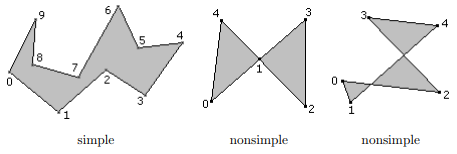
\includegraphics[scale=0.7]{nonsimpleExample}$$

\section{Related Work}
A similar project related to ours is "Fast Polygon Triangulation Based on Seidel's Algorithm" conducted by Atul Narkhede and Dinesh Manocha. As the title of the project suggests, the use of the Seidel's Algorithm was key. It uses the structure of undirected, unweighted, and connected graphs. It solves the problem in $O(n*logn)$ with polygons that do not have holes and using a query structure to locate a point in logarithmic time. This project approach was the following:
\begin{enumerate}
    \item Decompose the polygon in trapezoids. A \textbf{trapezoid} is a 4-sided flat shape with straight sides that has a pair of opposite sides parallel. This step is done by randomly selecting a segment from a set of segments that are non-horizontal and non-intersecting from the polygon and adding them incrementally to form the trapezoids inside the boundaries of the polygon.
    \item After the polygon is partitioned into trapezoids, they're yet again partitioned but this time into monotone polygons. \text{Monotone polygons} are polygons whose boundaries consist of two y-monotone chains. These \textbf{monotone chains} come from the Andrew's monotone chain convex hull algorithm. This algorithm constructs the convex hull of a set of 2-dimensional points and has a $O(nlogn)$ complexity. This step checks the segments from step 1 and see if the two vertices of each segment lie on the same side.
    \item The last step is to triangulate the monotone polygons. Their triangulation method was a greedy algorithm that cuts off the convex corners in a loop. The triangulation of each monotone polygon is done in $O(n)$.
\end{enumerate}
\cite{relatedProject}

\section{Computer Graphics}
The term "computer graphics" refers to anything involved in the creation or manipulation
of images on computer, including animated images.\cite{ComputerGraphics}. This is a very broad field, because it includes, for example, 2D and 3D images, such as animated images. For this paper we will be focused only on planar objects. Planar objects, sometimes called 2D shapes, are created on a single plane (usually the xy-plane). Focusing on planar objects, 2D primitives like lines, circles, etc. may be used to create more complex shapes.\cite{2DGraphics}. These graphics are often preferred over 3D because they give more control over the images, and it is very easy to escalate or rotate them.\\
Computer graphics first appeared in the 50's, and one of the firsts and more popular computer game was Spacewar!, developed at MIT by Steve Russell. It took the team about 200 man-hours to write the first version of Spacewar. Russell wrote Spacewar on a PDP-1, an early DEC (Digital Equipment Corporation) interactive mini computer which used a cathode-ray tube type display and keyboard input.\cite{SpaceWar}. Since then, 2D graphics have been being improved and now there are more and better algorithms and techniques that allow us easily keep developing 2D computer graphics.


\section{Polygon Triangulation}
Computing the triangulation of a polygon is a fundamental algorithm in computational
geometry. It also seems to be the most investigated partitioning method\cite{Triangulation}. \\Polygon Triangulation is the decomposition of a polygon in a surface or plane, into a set of triangles, with the restriction that each triangle side is entirely shared by two adjacent triangles. In computer graphics, polygon triangulation algorithms are widely used for tessellating curved geometries. Triangulation can be applied to both convex and concave polygons. Concave polygons are those that have internal angles greater than 180 degrees, convex polygons are the opposite, internal angles sum 180 or less degrees. The Triangulation Theorem \cite{Theorem}states that:
\begin{itemize}
    \item{Every simple polygon admits a triangulation}
\item{Every triangulation of an n-gon has exactly $n-2$ triangles}
\end{itemize}
$$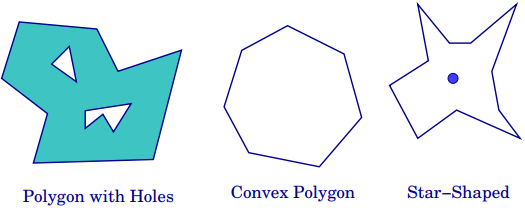
\includegraphics[scale=0.6]{Typeofpolygons}$$
\subsection{Triangulation Approaches}\cite{TriangulationApproaches}
    \subsubsection{\textbf{Non-Delaunay Algorithms}}
    \begin{itemize}
        \item{Greedy Triangulation}
        \item{Triangulation of Garey et.al}
        \item Ear Clipping / Ear Trimming
        \item{Radial Sweep}
    \end{itemize}
    \subsubsection{\textbf{Delaunay Algorithms}}
    \begin{itemize}
        \item Delaunay triangulation is proposed by B. Delaunay in 1934. Delaunay triangulation maximizes the minimum angles in triangles and avoids skinny triangles.
        \item Delaunay triangulation T of P is a triangulation of P such that the circum-circle of any triangle belonging to T does not contain points of P in its interior.
        \subsubsection{Properties}
        \begin{itemize}
            \item Local empty-circle property
            \item Max-min angle property
            \item Uniqueness
            \item Boundary property
        \end{itemize}
        \subsubsection{Algorithms}
        \begin{itemize}
            \item Incremental Algorithms
            \item Filliping Algorithm
            \item Plane Sweep Algorithm
            \item Divide and Conquer Algorithm
        \end{itemize}
    \end{itemize}
    

\section{Metodology}
\subsection{Delaunay Algorithms}
For  understanding  Deulanay  triangulation  algorithms  it  isnecessary an overview of Voronoi Diagrams.\\
A \textbf{ Voronoi diagram} is  on  of  the  simplest  way  for  making interpolation,  which  means  obtaining  new  data  points  within the  range  of  aleready  known  data  points.  Voronoi  diagrams,also known as Thiessen polygons, are used for partitioning the euclidean plane and it is done based on the euclidean distanceof a set of data points.The Voronoi diagram of a set of sites or generators (points) is a  collection  of  regions  that  divide  up  the  plane.  Each  region corresponds  to  one  of  the  sites  or  generators,  and  all  of  the points in one region are closer to the corresponding site thanto any other site. \cite{VoronoiD}. Thiessen polygons are used, for example,in  flights  for  finding  the  nearest  airport,  when  we  are  trying to  find  the  nearest  restaurants  and,  of  course,  in  computer graphics.\\In  figure  \ref{fig:VoronoiColored} you  can  see  an  example  of  Voronoi  cells  on  a colored  image.  Each  color  is  related  to  the  point  inside  the colored  section.  The  color  represents  the  section  of  the  map closer to that point than other data points of the plane.

\begin{figure}[H]
    \centering
    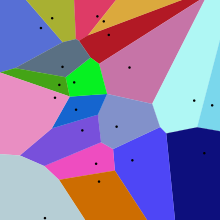
\includegraphics[width=150,height=150,keepaspectratio]{VoronoiColors.png}
    \caption{Voronoi Cells}
    \label{fig:VoronoiColored}
\end{figure}
    
It is very simple to understand how these regions are generated. Lets consider $P=\{P_1,P_2,...,P_n\}$ as a set of data points on a plane, $V={\{V_1,V_2,...,V_n\}}$ as lines connecting the points on the plane and finally $S={\{S_1,S_2,...,S_n\}}$ as the bisectors of each $V_i \in V$.Each section of the plane will be defined as the areas generated by the intersections of each $S_i$, as shown in figure \ref{fig:VoronoiDiagram1}. Black points represent data points $P_i$, black lines each $V_i$, as the lines connecting each data point, and red lines their bisectors that splits the map in tree sections. Each section is called a Voronoi Cell, and the whole sections together conforms the Voronoi Diagram.

\begin{figure}[H]
    \centering
    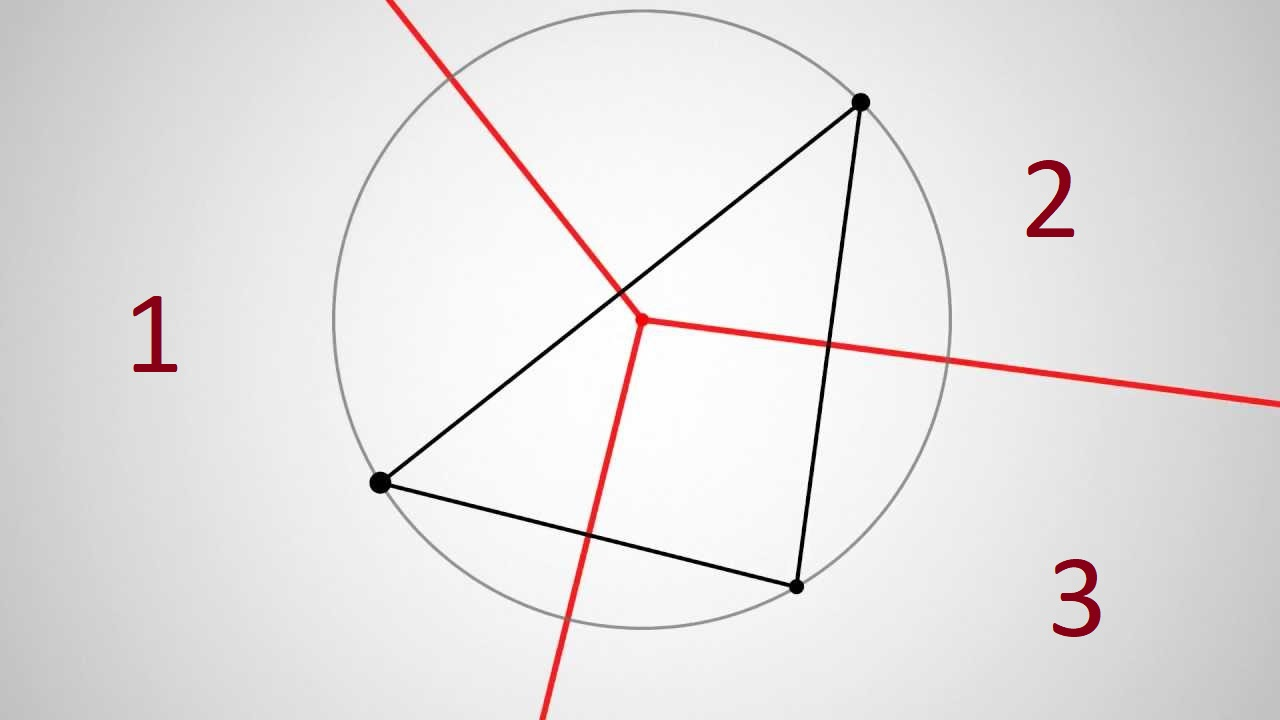
\includegraphics[width=200,height=150,keepaspectratio]{maxresdefault2.jpg}
    \caption{Simple Voronoi Diagram}
    \label{fig:VoronoiDiagram1}
\end{figure}

But, lets see how these diagrams are generated form scratch. First, we will place the data points. After that, it is necessary to draw lines connecting the data points. At the same time, we have to draw a bisector for each one of those lines. Finally, we "erase" the lines connecting the data points. The result will be the diagram.

\begin{figure}[H]
    \centering
    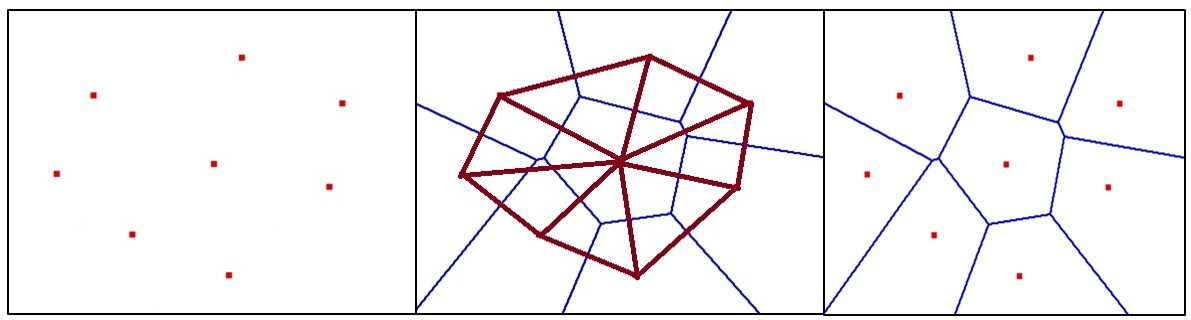
\includegraphics[width=200,height=100,keepaspectratio]{DiagramGeneration.jpg}
    \caption{Voronoi Diagram Generation}
    \label{fig:VoronoiDiagram1}
\end{figure}
    
\subsection{Ear Clipping}
An ear of a polygon is a triangle formed by three consecutive vertices $V_{i0},V_{i1},$ and $V_{i2}$ for which $V_{i1}$ is a convex vertex. The line segment from $V_{i0}$ to $V_{i2}$ lies completely inside the polygon, and no vertices of the polygon are inside the triangle other than its components. The line segment between $V_{i0}$ and $V_{i2}$ is a diagonal of the polygon. The vertex $V_{i1}$ is called the ear tip. A triangle has only one ear and can be any of the triangle's vertices. The Ear Clipping algorithm takes $O(n^2)$\cite{EarClipping}

\subsection{Code Analysis}
\begin{lstlisting}
    public void triangulatePolygon() {
      
        long start = System.currentTimeMillis(); //1
        boolean clockwise = isClockwise(points); //n
        int index = 0; //1
        if (points.size() < 3) { //1
            points.clear(); //1
        }else{
            while (points.size() > 2) { //n+1

              Point p1 = points.get((index + 0) % points.size());//1
              Point p2 = points.get((index + 1) % points.size());//1
              Point p3 = points.get((index + 2) % points.size());//1

            Vector v1 = new Vector(p2.x - p1.x, p2.y - p1.y);//1+1
            Vector v2 = new Vector(p3.x - p1.x, p3.y - p1.y);//1+1
                double cross = v1.cross(v2);//1+1
                Polygon triangle = new Polygon(); //1
                triangle.addPoint(p1.x, p1.y); //1
                triangle.addPoint(p2.x, p2.y); //1
                triangle.addPoint(p3.x, p3.y); //1

                if (!clockwise && cross >= 0 && validTriangle(triangle, p1, p2, p3, points)) { //1+n
                    points.remove(p2);//1
                    triangles.add(triangle);//1
                }
                else if (clockwise && cross <= 0 && validTriangle(triangle, p1, p2, p3, points)) { //1+n
                    points.remove(p2);//1
                    triangles.add(triangle);//1
                }
                else {
                    index++;//1
                }
            }
            long end = System.currentTimeMillis();//1
            long time = end-start;//1+1
            long minutes = (time / 1000)  / 60;//1+1
            long seconds = (time / 1000) % 60;//1+1
            long milli = time - (seconds * 1000) - (minutes * 60000);//1
            String report = "Time taken: " + minutes + " min " + seconds + " sec " + milli +" ms" ; //1
            JOptionPane.showMessageDialog(null,report);
        }
    }
\end{lstlisting}
triangulatePolygon Cost =
\newline
$(1)*19 +(2)*5+(n)+((n+1)*(1+n))$
\newline
$19+10+n+(n+n^2+1+n^2)$
\newline
$29+n+(n^2+n+1)$
$30+n+n^2$
$$\therefore O(n^2)$$
\begin{lstlisting}
    def addPoint(self, p):
    
        p = np.asarray(p) // 1+1
        idx = len(self.coords) //n
        self.coords.append(p)//1

        bad_triangles = []//1
        for T in self.triangles: //n
            if self.inCircleFast(T, p)://1
                bad_triangles.append(T)//1
        boundary = []//1
        T = bad_triangles[0]//1
        edge = 0 //1
        while True://n+1
           
            tri_op = self.triangles[T][edge]//1
            if tri_op not in bad_triangles://1
                boundary.append((T[(edge+1) % 3], T[(edge-1) % 3], tri_op)) //1+1+1+1
                edge = (edge + 1) % 3 //1+1+1

                if boundary[0][0] == boundary[-1][1]://1
                    break//1
            else:
                edge = (self.triangles[tri_op].index(T) + 1) % 3//1+1+1
                T = tri_op//1
        for T in bad_triangles://n
            del self.triangles[T]//1
            del self.circles[T]//1
        new_triangles = []//1
        for (e0, e1, tri_op) in boundary://n
            T = (idx, e0, e1)//1
            self.circles[T] = self.circumcenter(T)//n
            self.triangles[T] = [tri_op, None, None]//1
            if tri_op://1
                for i, neigh in enumerate(self.triangles[tri_op])://n
                    if neigh://1
                        if e1 in neigh and e0 in neigh://1
                            self.triangles[tri_op][i] = T//1
            new_triangles.append(T)//1
        N = len(new_triangles)//n
        for i, T in enumerate(new_triangles)://n
            self.triangles[T][1] = new_triangles[(i+1) % N] //1+1  
            self.triangles[T][2] = new_triangles[(i-1) % N]  //1+1
\end{lstlisting}
addPoint Cost = 
\newline
$(1)*6+2+n+n+(n+1)*15+(n)*2+n(3+n(3))+n+n(4)$
\newline
$6+2+2n+(15n+15)+2n+n(3+3n)+n+4n$
\newline
$8+2n+15n+15+2n+3n+3n^2+5n$
\newline
$3n^2+25n+23$
$$\therefore O(n^2)$$
\section{Experiments}
For the experimentation process, a background image was set to be used as a guideline and then manually, add vertices in order to enclose the image and create similar polygons with different vertices, and watch how the algorithm behaves and how his time can change depending on the quantity of his vertices.

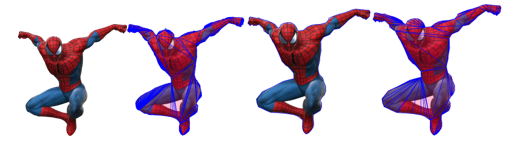
\includegraphics[scale=0.6]{spideyresults.png}

In this experiment it can be seen that in the SpiderMan image it test with different quantity of vertices, and according to that the quantity of triangles will be n-2, and because that the algorithm will last more and will increase his response time theoretically.

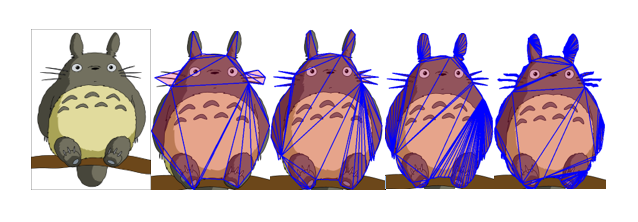
\includegraphics[scale=0.53]{totoroResults.png}

Also with this last image of Totoro, according to the quantity of vertices it will be the quantity of the triangles, and with this said and theoretically seen in the previous analysis of the triangulation code it should extend his duration time with more vertices.

\section{Results}

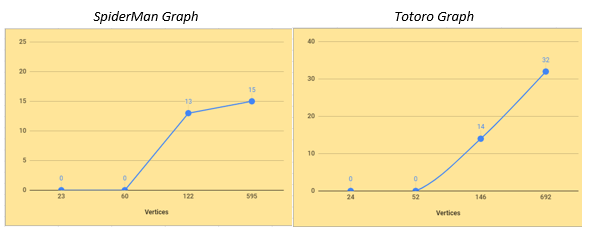
\includegraphics[scale=0.58]{Graphs.png}

After conducting this part of the experiment, the results showed that the amount of vertices versus time can be different across different polygons based on the contour of the images. This is because there are images that, after enclosing them in a convex hull formed by the vertices, can be simple polygons more than others, that is, that have more edges, bends, curves, etcetera. So, the algorithm needs to check if the new triangle formed by the inclusion of a new vertex is a valid one or not. In synthesis, if a polygon has a lot of vertices, that means that the algorithm will take more time testing each of its vertices; therefore, taking more time to triangulate said polygon. In the last figure shows the graph corresponding to the Totoro image test, and can give a glimpse of the $n^2$ behaviour even though the line is not very steep.\\

\bibliographystyle{plain}
\bibliography{references}
\end{document}

